\documentclass[12pt, titlepage]{article}

\usepackage{fullpage}
\usepackage[round]{natbib}
\usepackage{multirow}
\usepackage{booktabs}
\usepackage{tabularx}
\usepackage{graphicx}
\usepackage{float}
\usepackage{hyperref}
\usepackage{longtable}
\usepackage{caption}
\hypersetup{
    colorlinks,
    citecolor=blue,
    filecolor=black,
    linkcolor=red,
    urlcolor=blue
}

%% Comments

\usepackage{color}

\newif\ifcomments\commentstrue %displays comments
%\newif\ifcomments\commentsfalse %so that comments do not display

\ifcomments
\newcommand{\authornote}[3]{\textcolor{#1}{[#3 ---#2]}}
\newcommand{\todo}[1]{\textcolor{red}{[TODO: #1]}}
\else
\newcommand{\authornote}[3]{}
\newcommand{\todo}[1]{}
\fi

\newcommand{\wss}[1]{\authornote{blue}{SS}{#1}} 
\newcommand{\plt}[1]{\authornote{magenta}{TPLT}{#1}} %For explanation of the template
\newcommand{\an}[1]{\authornote{cyan}{Author}{#1}}

%% Common Parts

\newcommand{\progname}{Mechatronics} % PUT YOUR PROGRAM NAME HERE
\newcommand{\authname}{Team \#20, Team Name
\\ Robert Zhu zhul49
\\ Zifan Meng mengz17
\\ Jiahui Chen chenj194
\\ Kelvin Huynh huynhk12
\\ Runze Zhu zhur25
\\ Mirza Nafi Hasan hasanm21} % AUTHOR NAMES                  

\usepackage{hyperref}
    \hypersetup{colorlinks=true, linkcolor=blue, citecolor=blue, filecolor=blue,
                urlcolor=blue, unicode=false}
    \urlstyle{same}
                                


\newcounter{acnum}
\newcommand{\actheacnum}{AC\theacnum}
\newcommand{\acref}[1]{AC\ref{#1}}

\newcounter{ucnum}
\newcommand{\uctheucnum}{UC\theucnum}
\newcommand{\uref}[1]{UC\ref{#1}}

\newcounter{mnum}
\newcommand{\mthemnum}{M\themnum}
\newcommand{\mref}[1]{M\ref{#1}}

\begin{document}

\title{System Design for \progname{}} 
\author{\authname}
\date{\today}

\maketitle

\pagenumbering{roman}

\section{Revision History}

\begin{tabularx}{\textwidth}{p{3cm}p{2cm}X}
\toprule {\bf Date} & {\bf Version} & {\bf Notes}\\
\midrule
January 18, 2023 & 1.0 & Initial System Design Draft\\
March 23, 2023 & 1.1 & Update Timeline\\

\bottomrule
\end{tabularx}

\newpage

\tableofcontents

\newpage

\listoftables

\listoffigures

\newpage

\pagenumbering{arabic}

\section{Introduction}
The purpose of this document will give an overview of the system components for how the user interacts with the system, 
and the communication between the design of the hardware, software, and any electrical components.

\section{Purpose}
The purpose of our project is to create a device that will translate sign language gestures into their corresponding words 
or phrases. This will require the creation and development of a computer vision system alongside a machine learning model that 
will be used to recognize the hand motions, as well as a Raspberry Pi that will speak the word or phrase. The user will perform 
the sign language motion that will be captured by our computer vision system through a camera, and processed by our machine learning 
model and spoken through our Raspberry Pi.


\section{Scope}
OpenASL is primarily designed to assist the hearing impaired who use sign language to communicate. The following goals listed 
describe the key requirements for OpenASL to efficiently translate gestures and motions for any individual who does not know sign language 
to understand. More detailed explanations for each goal can be found in the SRS (REF SRS 2.2.1).

\begin{figure}[H] 
\centering
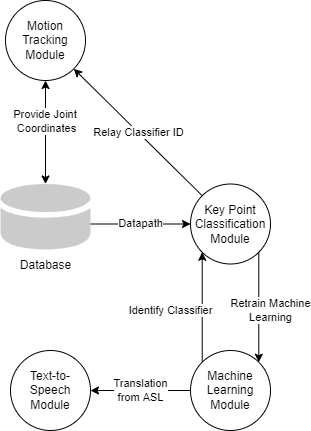
\includegraphics[width=\textwidth,height=0.88\textheight,keepaspectratio,scale=0.75]{SystemContextDiagram.jpg} 
\caption{System Context Diagram} 
\label{Fig.System_Context_Diagram} 
\end{figure}

\begin{center}
\begin{tabular} {m{18em}}
  \toprule		
  \textbf{Goals}\\
  \midrule 
  Reliable and Accurate Translations\\
  \hline
  Real Time Translations\\ 
  \hline
  Ease of Use\\
  \hline
  Affordability\\
  \hline
  Customizable to User\\
  \bottomrule
\\
\captionof{table}{Project Goals}
\end{tabular}
\end{center}
\section{Project Overview}

\subsection{Normal Behaviour}
OpenASL acts as a medium for sign language to spoken language to help the hearing impaired communicate without the need of a human translator. 
Under normal operations, the user would perform ASL gestures in front of a camera that would detect motion, which would begin having the Raspberry Pi 
start classifying the movement of the user with its database and output the corresponding English word/phrase through speakers for the other person to 
understand. The user is also able to train the algorithm to learn any of the user’s subtle differences in gestures from the standard ASL language to 
improve the accuracy of classification for words/phrases.

\subsection{Undesired Event Handling}
In the event of an undesired error during the translation, the system should stop the translation being spoken through the speaker and display on the 
user interface that an error has occurred to let the user know that something has happened to the system. In the case that an error occurs during the 
process of the user training the model, such that the system is unable to classify the gesture, an error message should display on the interface to 
tell the user to retry. This would help prevent any incorrect data from being entered into the classification database for more accurate results.

\subsection{Component Diagram}

\begin{figure}[H] 
\centering
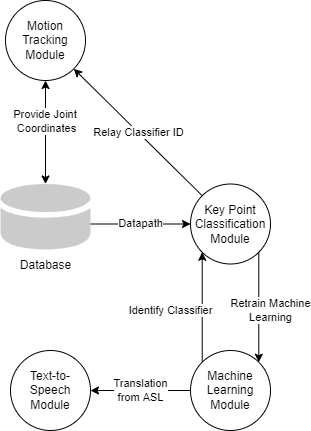
\includegraphics[width=\textwidth,height=0.88\textheight,keepaspectratio]{ComponentDiagram.jpg} 
\caption{Component Diagram} 
\label{Fig.Component_Diagram} 
\end{figure}

\subsection{Connection Between Requirements and Design} \label{SecConnection}
(REF SRS 6.1, 6.2, 8.1, 8.2, 8.3, 8.4 for description of ID).

\renewcommand{\arraystretch}{1.2}
\noindent \begin{longtable}{p{0.2\textwidth}|p{0.75\textwidth}}
\hline
\textbf{Requirement ID} & \textbf{Design Decision}\\
\hline
CFR1
& We used a Tensorflow machine learning algorithm already incorporated into the Mediapipe library to recognize hand shape and model its joints through the lens of any camera when it detects motion.\\
\hline
CFR2
& The program normalizes the resolution of any camera lens to ensure that the coordinates detected from the camera can be used to classify the vision of a gesture to its corresponding word/phrase.\\
\hline
MLFR1
& We used a Tensorflow machine learning algorithm already incorporated into Mediapipe to recognize a hand shape and model its joints. This allows the coordinates of each joint to be identified and recorded into a dataset for the system.\\
\hline
MLFR2
& Using the Mediapipe library, we have set up our program to take a set of normalized coordinates based on the location of the hand. This allows us to recognize.\\
\hline
MLFR3
& The Mediapipe library has a built-in variable to limit the number of hands that can be tracked. We have limited that number to 2.\\
\hline
MLFR4
& We acquired a Raspberry Pi board that we would use to process the machine learning model and set the delay within the hand tracking script to a reasonable amount for conversation.\\
\hline
MLFR5
& Mediapipe’s built-in machine learning model classifies hand shapes within a specified confidence value between 0 and 1, of which a defaulted value of 0.5 is used. This means that if the model can confidently say with 50\% certainty that the video/image being recorded contains a hand, the hand and its joints will be displayed (subject to hand limit defined by MLFR3).\\
\hline
MLFR6
& The Raspberry Pi board has the necessary hardware to process the hand gestures at a pace that is understandable to other people.\\
\hline
MLFR7
& The program is set up with a training mode, where we can add data points for certain gestures to increase the accuracy of the model.\\
\hline
NFR1
& The Keypoint Classifier Module checks the dataset for each gesture and is able to display its confidence as a percentage for an estimate of how often it will be able to classify the correct gesture to support testing.\\
\hline
NFR2
& Mediapipe, an open-source library built from OpenCV for Python, is able to detect the user’s hands and highlight their joints accordingly to help the user focus on their hand gestures.\\
\hline
NFR3
& The device is already preset with a dataset that contains many common phrases that can be translated, allowing for little set up.\\
\hline
NFR4
& The user interface contains only written words and is clearly labeled for translating (normal operation), and can be further adapted into training the machine learning model as incorrect classifications indicate that the model must be retrained.\\
\hline
NFR5
& The Motion Tracking module is equipped with the ability to snapshot hand positions as needed to train the relevant classifier label if retraining is needed. These coordinates are then stored into a .csv file which can be used in conjunction with the Keypoint Classifier module to retrain the model.\\
\hline
NFR6
& We have chosen to implement our program onto a Raspberry Pi board. The board has a small form factor, making it easy to carry and very portable.\\
\hline
NFR7
& The current design is using the universal training model for standard ASL gestures. And the machine learning function for the program will allow for the ease of training in different grammar and phonology in the future.\\
\hline
\caption{Requirements and Design Decisions}
\end{longtable}

\renewcommand{\arraystretch}{1.2}
\noindent \begin{tabularx}{\textwidth}{p{0.2\linewidth}|p{0.72\linewidth}}
\toprule
\textbf{Module} & \textbf{Requirements}\\
\midrule
Motion Tracking
& CFR1, CFR2, MLFR1, MLFR2, MLFR3, MLFR5, MLFR6, NFR2\\
\hline
Keypoint Classifier
& NFR1, NFR5\\
\hline
Machine Learning
& MLFR4, MLFR7\\
\bottomrule
\end{tabularx}
\captionof{table}{Modules and Requirements}

\section{System Variables}
\subsection{Monitored Variables}

\renewcommand{\arraystretch}{1.2}
\noindent \begin{tabularx}{\textwidth}{p{0.15\linewidth}|p{0.12\linewidth}|p{0.12\linewidth}|p{0.5\linewidth}}
\toprule
\textbf{Monitor Name} & \textbf{Monitor Type} & \textbf{Range} & \textbf{Description}\\
\midrule
mode & Integer & [0, 2] & Program operation mode (normal, keypoint training, point history/motion training)\\
\hline
num & Integer & [0,25] & Determines corresponding ASL classifier label to use\\
\hline
landmark\_list & List & [-1.0,1.0] & Set of normalized coordinates to be paired with ASL classifier label\\
\bottomrule
\end{tabularx}
\captionof{table}{Monitored Variables}

\subsection{Controlled Variables}

\renewcommand{\arraystretch}{1.2}
\noindent \begin{tabularx}{\textwidth}{p{0.2\linewidth}|p{0.12\linewidth}|p{0.12\linewidth}|p{0.45\linewidth}}
\toprule
\textbf{Control Name} & \textbf{Control Type} & \textbf{Value} & \textbf{Description}\\
\midrule
RANDOM\_SEED & Integer & 51 & Value set to control random shuffling in ML model for reproducible output\\
\bottomrule
\end{tabularx}
\captionof{table}{Controlled Variables}

\subsection{Constants Variables}

\renewcommand{\arraystretch}{1.2}
\noindent \begin{tabularx}{\textwidth}{p{0.28\linewidth}|p{0.12\linewidth}|p{0.08\linewidth}|p{0.4\linewidth}}
\toprule
\textbf{Constant Name} & \textbf{Constant Type} & \textbf{Value} & \textbf{Description}\\
\midrule
min\_detection\_confidence & Integer & 0.5 & Minimum confidence for hand detection from tracking script\\
\hline
num & Integer & 0.5 & Minimum confidence for hand joint tracking\\
\hline
landmark\_list & Integer & 16 & Maximum point history entries for motion tracking\\
\hline
NUM\_CLASSES & Integer & 26 & Number of classifier labels in ML model\\
\bottomrule
\end{tabularx}
\captionof{table}{Constant Variables}

\section{User Interfaces}

The user interface is designed to give the user the choice between translating ASL to spoken language and training the machine learning module to adapt 
to any of the user’s habits for any phrases. For translating ASL, the user would interact with the Raspberry Pi Camera that is equipped to register hand 
movement for the machine learning algorithm to classify. Either on a PC or laptop, the English translation will be provided to the user to determine if 
it is accurate or if it requires additional training. For training, the interface will display when to do the gesture in front of the camera to retrain 
the classification module for more accurate results. For the audience, who do not know sign language, a text-to-speech module will deliver a translation of ASL.

\section{Mechanical Hardware}

For our project, we will be implementing our program onto a Raspberry Pi 3 Model B+ board. We chose a Raspberry Pi board mainly because of its smaller form 
factor. We wanted our device to be portable, but we also need enough processing power to run a machine learning algorithm. The Raspberry Pi board allows us 
to achieve both of these goals. The Raspberry Pi board also has the ability to add external components such as a speaker and camera, both of which will be 
needed for our project. We will be using the Raspberry Pi Camera v2 to capture the sign language gestures, and we will use the on-board audio socket to output 
the translation.

Raspberry Pi 3 Model B+
GPU: Broadcom Videocore-IV
Memory: 1 GB
Storage: Micro-SD
Ports: 3.5mm analogue audio-video jack, Camera Serial Interface (CSI)

\begin{figure}[H] 
\centering
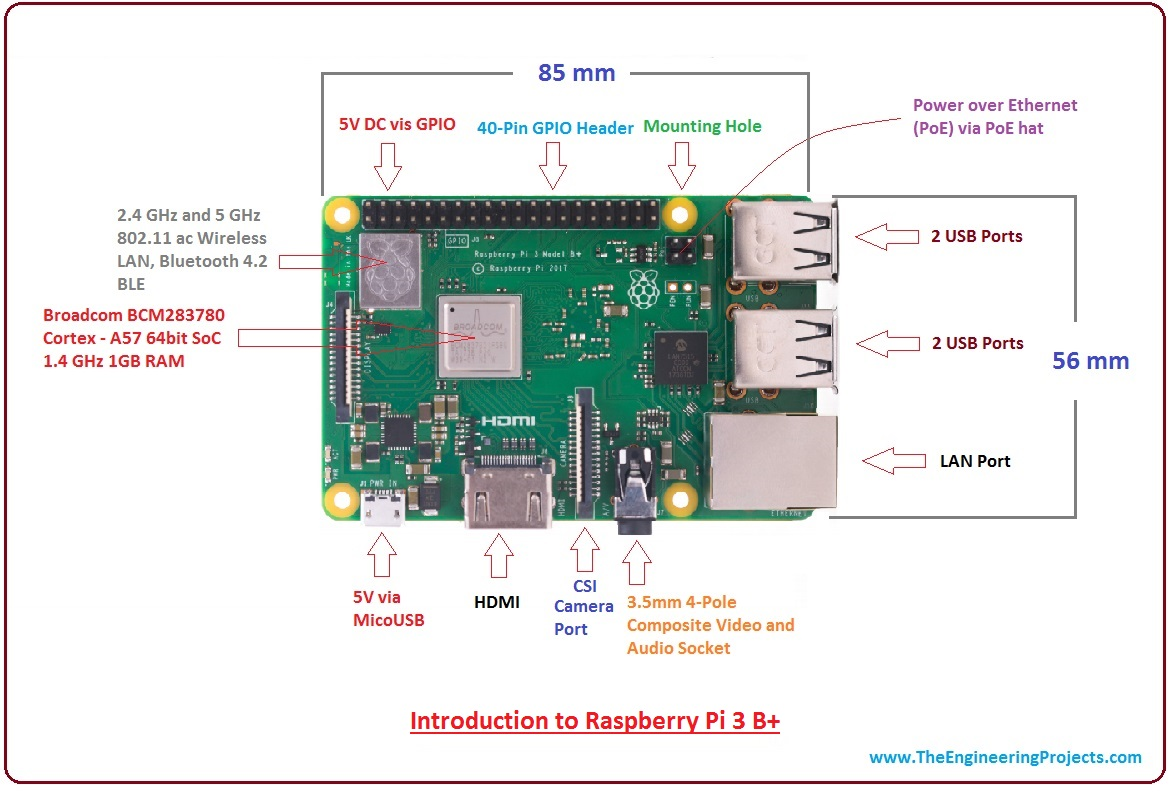
\includegraphics[width=\textwidth,height=0.88\textheight,keepaspectratio]{PiBoard.jpg} 
\caption{Raspberry Pi Model 3 B+ diagram} 
\label{Fig.Pi_Board} 
\end{figure}

Raspberry Pi Camera v2
Video Resolution: 1080p30, 720p60 and 640x480p60/90
Sensor: Sony IMX219 Image sensor

\section{Design of Electrical Components}

N/A

\section{Design of Communication Protocols}

N/A

\section{Timeline}

\renewcommand{\arraystretch}{1.2}
\noindent \begin{tabularx}{\textwidth}{p{0.3\linewidth}|p{0.3\linewidth}|p{0.35\linewidth}}
\toprule
\textbf{Objective} & \textbf{Date to be completed by} & \textbf{Member(s) Responsible}\\
\midrule
Create an interface that lets the user switch between training and translating & Jan 20, 2023 & Nafi Hasan\\
\hline
Add an expanded vocabulary of common phrases into the database (initial database) & Jan 31, 2023 & Robert Zhu, Jiahui Chen\\
\hline
Build and connect Raspberry Pi to OpenCV system to provide real-time translation & Feb 5, 2023 & Zifan Meng\\
\hline
Hardware testing after constructing and connecting Raspberry Pi with the program & Feb 5, 2023 & Zifan Meng\\
\hline
Program a text-to-speech algorithm & Feb 5, 2023 & Runze Zhu, Zifan Meng\\
\hline
Testing the whole program on computer & Feb 6, 2023 & Robert Zhu\\
\hline
Move OpenCV system and machine learning model onto Raspberry Pi & Feb 6, 2023 & Kelvin Huynh\\
\hline
Testing the Raspberry Pi with OpenCV system and machine learning model & Feb 06, 2023 & Kelvin Huynh, Robert Zhu\\
\hline
Software improvement and modification after testing & Feb 07, 2023 & All group members\\
\hline
Database implementation and testing to include more vocabularies and phrases & Feb 08, 2023 & Jiahui Chen, Robert Zhu\\
\hline
Rev 0 Demo & Feb 09 & All group members\\
\bottomrule
\end{tabularx}
\captionof{table}{Objectives Timeline}

% \bibliographystyle {plainnat}
% \bibliography{../../../refs/References}

\newpage{}

\appendix

%\section{Interface}

%\section{Mechanical Hardware}

%\section{Electrical Components}

%\section{Communication Protocols}

\section{Reflection}

The information in this section will be used to evaluate the team members on the
graduate attribute of Problem Analysis and Design.  Please answer the following questions:

\begin{enumerate}
  \item What are the limitations of your solution?  Put another way, given
  unlimited resources, what could you do to make the project better? (LO\_ProbSolutions)
  ~\\
  \\
  Robert Zhu: One of the limitations for our solution is that it is unable to capture the full language of ASL through only capturing hand gestures. 
  That is because ASL often uses a range of different body movements to deliver a proper sentence. For example, the phrase for “come here” involves 
  tapping the knee, which our program is unable to categorize since it only tracks hand movement. Grammar is also an issue as face expressions dictate 
  the tone, urgency, and even the meaning of phrases when combined with hand gestures. At the moment, these aspects of ASL are out of the scope for the 
  current plan, however, with enough time and datasets from the ASL community that the machine learning algorithm can read from, more of this language 
  can be translated.
  \\
  ~\\
  \\
  Kelvin Huynh: Another limitation for our solution is that depending on the size of the subset of ASL that we incorporate into the design, there may or 
  may not be sufficient space available on the Raspberry Pi to accommodate our design. This is detrimental to being able to properly expand the amount of 
  ASL able to be translated. At the moment the scope does not encompass being able to translate the entirety or a large portion of ASL, so this limitation 
  is fine to work around.
  \\
  ~\\
  \\
  Runze Zhu: One other limitation for our solution is the amount of time it takes to capture each character and translate some long sentences. Currently, it is set up in a way that requires the user to perform the hand signs one by one and hold each sign for sometime as  it takes some time to translate each sign. If the user needs to express long sentences, it would be very time consuming. At the moment, improving the speed of translation is not on the plan, while more hot words of body language can be created with enough time, so the translation can be more efficient.
   \\
  ~\\
  \\
  Zifan Meng: One of the limitations of our solution is we cannot provide customization to each individual user. Every user has their own habits about
  hand gestures, for our current solution, we only have a universal training model for standard ASL gestures, if a user’s hand gesture differs a lot 
  from the standard ASL gesture, it is likely that the translation is incorrect. If we were to have more development time, we could develop a user accounts
  function, each user has their own account and their own database, some specific gestures of theirs can be stored in the database and the product is 
  able to translate accordingly to the account that’s logged in.
  \\
   ~\\
  \\
    Mirza Nafi Hasan: One limitation of our solution is the amount of time it takes to train our machine learning model. Currently, we have it set up in a way 
that requires someone to perform the hand sign and record it themselves. Since there are no machine learning models that have data on different sign language
gestures, if we want to be able to translate all of ASL, that will require someone to perform every gesture in sign language, which would be a very time 
consuming process. If we had unlimited resources, we could have someone who is very familiar with ASL do these gestures, or we could try to find a way to
automate the training process.
  \\
  ~\\


  Jiahui Chen: In addition, another limitation for the solution is that the database for the ASL translator needs to be constantly updated. Since new English words and phrases are created every year and as mentioned previously, the database cannot update by itself. And the programmers need to take time to gather all the new words and phrases created every year and enter the program to train the translator. 
  \\
  ~\\
 \\
  
  \item Give a brief overview of other design solutions you considered.  What
  are the benefits and tradeoffs of those other designs compared with the chosen
  design?  From all the potential options, why did you select documented design?
  (LO\_Explores)
  ~\\
  \\
  Robert Zhu: One other design solution involved designing a device that is placed on the hands of the user with sensors that are capable of capturing 
  hand gestures, and transmitting the information into a spoken language. The main benefit of this method compared to our current chosen design would 
  be a very high accuracy in being able to classify the motion. Having sensors on each joint would provide more information for the processing unit by 
  being able to distinctly tell the position of each finger, leading to fewer mistakes compared to using a camera sensor. We did not select this method 
  as it greatly reduced the scope of ASL to only having finger movements. ASL uses dynamic motion that can not be captured using glove sensors, while a 
  camera sensor is able to detect these movements and classify them. A dataset is also easier to gather through using a camera sensor as the hardware 
  required for gloves requires a lot of effort to generate enough datasets to accurately translate.
  \\
  ~\\
  \\
  Kelvin Huynh: One design solution involved using glasses to translate ASL for someone with no understanding of ASL. This would have used the same solution 
  as the current design using computer vision. However from a design standpoint, this solution doesn’t have a lot of benefit as it means that the end-user 
  fits a very specific niche as those who are exposed to ASL on a daily basis (i.e those who are hard of hearing) would have no use for such a solution as they 
  already understand the meaning of the different signs. The design we chose enables not only personal usage, but wider application to a teaching setting as 
  well since in theory the device can be hooked up to a large scale display device if needed.
  \\
  ~\\
  \\
  Runze Zhu: Another design solution we considered was developing an application that can be installed on cell phones or laptops to replace the Raspberry Pi, which can detect ASL language with cameras of those devices and output the results by audio or showing the words on the screen. Some advantages of such design solution would be it can use scalable cloud storage for training and saves the cost of extra hardware such as Raspberry Pi and extra camera. It’s also more portable since users don’t need to carry those hardware for translation. However, it would be quite hard to develop a software that can fit in various hardware and might need a server to run the machine learning algorithm and send the results to the users, which can be quite expensive.
  \\
  ~\\
  \\
  Zifan Meng: One design solution we considered was implementing a LED screen on Raspberry Pi that outputs the translation results. Our current solution 
  is to have a speaker for audio output, if we have both visual output and audio output, the device is more complete as a portable, individually-working 
  device, and is suitable for all users (users with other disabilities). However this solution significantly increases the complexity of the design and 
  increases the cost of the device. The design that we have right now is for educational purposes or to help other people to understand people with hearing disabilities, 
  hence the audio output is sufficient enough for helping most of the users to understand ASL languages.
  \\
  ~\\
  \\
    Mirza Nafi Hasan: One other design solution we considered was instead of using a Raspberry Pi board, we considered using a smartphone. Some advantages of 
    this design solution would be that it satisfies the portability requirement we were aiming for. This would also be very accessible considering that everyone
    has a phone these days. Almost all smartphones have a camera and a speaker meaning we can capture the ASL gestures as input and output the translation 
    through the speaker. We decided against this design because we were unsure whether the average smartphone would be able to run a machine learning algorithm
    on it. Also, creating a program for one set of hardware would be easier to manage since many things can go wrong if we wanted to test our program on 
    multiple types of hardware.
    \\
    ~\\
    \\
  Jiahui Chen: Another design option can be using a laptop to replace the Raspberry Pi to detect the hand gestures by the laptop's camera and output the results by audio. The advantages of this solution are there is no extra hardware such as Raspberry Pi and camera required to detect the hand motion. Only the laptop is needed to fulfill the whole translation process. And since many events are held virtually now, the ASL translation system that is created on laptops can be used directly by the users and the translator does not have to stay in the meeting for the whole time to do the translation work. Also having the design option on laptops, more people are able to access the program to gain benefits from using it since it does not involve buying extra equipment. We did not choose this option because the laptop is big and it is hard to  bring it everywhere we go to do the translation work compared to a Raspberry Pi board. And our selected design is more flexible for in-person conversation.  
  \\
\end{enumerate}

\section*{References}
Raspberry pi documentation Raspberry Pi hardware. Available at: https://www.raspberrypi.com/documentation/computers/raspberry-pi.html (Accessed: January 17, 2023). 
\bibliographystyle {plainnat}
\bibliography{../../../refs/References}

\end{document}
